\documentclass[conference]{IEEEtran}
\IEEEoverridecommandlockouts
% The preceding line is only needed to identify funding in the first footnote. If that is unneeded, please comment it out.

\usepackage{cite}
\usepackage{amsmath,amssymb,amsfonts}
\usepackage{algorithmic}
\usepackage{graphicx}
\usepackage{textcomp}
\usepackage{xcolor}
\usepackage{tabularx}
\usepackage{graphicx}
\usepackage{comment}
\usepackage[utf8]{inputenc}
\graphicspath{ {Imagenes/}}
\def\BibTeX{{\rm B\kern-.05em{\sc i\kern-.025em b}\\kern-.08em
    T\kern-.1667em\lower.7ex\hbox{E}\kern-.125emX}}
\usepackage{float}
\newcommand\tab[1][1cm]{\hspace*{#1}}
\begin{document}

\title{Modelo LSTM de predicción de éxito de las ventas para empresas B2B}


\author{
    \IEEEauthorblockN{1\textsuperscript{st} Matos Manguinuri, Steve Sader}
    \IEEEauthorblockA{\textit{Facultad de Ingeniería de Sistemas e}\\
        \textit{Informática} \\
        \textit{Universidad Nacional Mayor de San}\\
        \textit{Marcos}\\
        Lima, Perú \\
        steve.matos@unmsm.edu.pe}
    \and
    \IEEEauthorblockN{2\textsuperscript{st} Pastor Guerrero, Diego Alejandro }
    \IEEEauthorblockA{\textit{Facultad de Ingeniería de Sistemas e}\\
        \textit{Informática} \\
        \textit{Universidad Nacional Mayor de San}\\
        \textit{Marcos}\\
        Lima, Perú \\
        diego.pastor@unmsm.edu.pe}
    \and
    \IEEEauthorblockN{3\textsuperscript{st} Taipe Carrión, Erick Rafael Camilo }
    \IEEEauthorblockA{\textit{Facultad de Ingeniería de Sistemas e}\\
        \textit{Informática} \\
        \textit{Universidad Nacional Mayor de San}\\
        \textit{Marcos}\\
        Lima, Perú \\
        erick.taipe@unmsm.edu.pe}
    \and
    \IEEEauthorblockN{1\textsuperscript{st} Postigo Vega, Abel Sebastian }
    \IEEEauthorblockA{\textit{Facultad de Ingeniería de Sistemas e}\\
        \textit{Informática} \\
        \textit{Universidad Nacional Mayor de San}\\
        \textit{Marcos}\\
        Lima, Perú \\
        abel.postigo@unmsm.edu.pe}
}

\maketitle

\begin{abstract}
 El propósito de esta investigación es construir un modelo de predicción de ventas para empresas orientada a servicios utilizando el enfoque 
 de deep learning, que ha ganado una atención significativa en los últimos años. El presente estudio utiliza datos de ventas de una empresa privada 
 llamada Seminarium Peru, en el cual los datos están un rango 3 años de antigüedad (40292 instancias) de lo cual servirá para construir un modelo 
 de predicción de ventas que, dadas las variables mas relevantes de una venta en particular, predice el éxito de esta venta. Por lo que en 
esta investigacion proponemos el diseño de un modelo LSTM y de ahí se validará el dataset de la empresa de esta investigación lo cual 
logró una tasa de error cuadrático medio de predicción de venta de 0.0200.\end{abstract}
\begin{IEEEkeywords} 
     Modelo Hibrido, Prediccion de Ventas, LSTM, Empresas B2B.
\end{IEEEkeywords}

\section{Introduccion}
Realizando una revisión a las literaturas sobre la predicción de ventas y predicción de clientes, en los últimos años ha habido varias 
investigaciones que buscaron nuevos métodos y formas de resolver el problema de la predicción de ventas y de predicción de clientes de 
forma separada. Para la de predicción de ventas se usaron modelos como ARIMA pero ese modelo de forma individual ha sido descartado 
últimamente por su falta de precisión al ser solo un modelo estadístico , y donde actualmente otras investigaciones proponen 
modelos usando deep learning \cite{b1} \cite{b2} , fusiones de técnicas \cite{b3} \cite{b4}, nuevo modelos basados en Deep learning \cite{b5} 
\cite{b6} \cite{b7}, frameworks \cite{b8} y arquitecturas \cite{b9} para la predicción de ventas . También en los últimos años se ha tomado en 
cuenta la predicción de clientes \cite{b10} \cite{b11} \cite{b12} \cite{b13} \cite{b14} como una gran oportunidad para mejorar el flujo de ventas.\\

En la investigación \cite{b7} aplicaron un modelo de clasificación bayesiana usando TAN Bayes pero solo usaron las variables más relevantes y 
finales de la venta, mas no usaron variables como las del cliente o las variables de todo un flujo de ventas, lo cual permitiría mejorar la 
predicción no solo de la venta sino también la predicción de la demanda que en este caso es de la empresa HP.\\

Indica un modelo hibrido entre ARIMA y RNN\cite{b4} que puede mejorar la predicción de las ventas diarias de una forma abismal y la dataset 
de apple que usaron pesar de que tenía cantidad decente de datos (6758 para ser más exactos),a parte que era de dominio público, solo 
tenía data con dos atributos( fecha diaria, la cantidad de dinero que se vendió ese día), por cada instancia pero no tomo en cuenta otras 
variables presentes en una venta como la actividad económica del cliente , tipos de productos que se vendieron , entre otros que se 
usaran en esta investigación y también el data set no es de un ambiente real, por ende, su aplicación no hace un aporte de manera exacta a 
la investigaciones de los modelos de predicción de venta\\

También en otras investigaciones como \cite{b15} solo se prioriza la predicción de ventas en periodos mensuales , lo cual es un rango grande 
para poder determinar las ventas y con lleva a que la predicción de ventas sea algo obsoleta porque la predicción de ventas se debe tratar de 
hacer en el rango más corto posible para poder tomar decisiones más efectivas y rápidas tanto a nivel administrativo como a nivel de áreas 
comerciales , además que incluso teniendo información del ERP que comenta en \cite{b15} se podría aplicar con más precisión la predicción de 
la venta en una rango mucho menor ( por ejemplo de forma diaria ) usando las variables que almacena el ERP , que lo más seguro , en experiencia 
de este lector de uso de ERPS , contendrá variables sumamente importantes del cliente y del flujo de la venta y que se usaría para mejorar 
la precisión, por lo que es posible incluso hacer predicciones individuales de cada venta.\\

Muchas empresas sufren un síndrome crónico en el que sus pronósticos de CRM se convierten en un registro histórico y no en una guía para el 
futuro \cite{b16}, estos datos al final se desperdician y no se usan para futuras predicciones de las próximas ventas.\\

Con inteligencia artificial (IA) y aprendizaje automático (ML), las marcas y las agencias pueden proporcionar los datos correctos a la persona 
adecuada en el momento adecuado. Estas tecnologías permiten métodos automatizados y escalables para unir las fuentes de datos y luego proporcionar 
información sobre cómo y dónde el usuario lo necesita \cite{b17} , por ende, aplicar IA y ML al mundo de los negocios es una de las mejores ideas 
en cuestión de saber si tu producto y/o servicio está dando los resultados que esperabas.\\

Si bien la mayoría de los especialistas en marketing son expertos en leer informes y métricas estándar, pocos están capacitados para analizar datos 
de múltiples fuentes con la suficiente profundidad para informar mejores decisiones de negocios \cite{b17} , esto impide que sea difícil para el 
área de marketing puedan interpretar fácilmente la gran cantidad de datos que sea vengan de varias fuentes y da por consecuencia que el área de 
ventas es las más perjudicada con este decisión puesto que ellos son la parte operatoria y provocara que su área tenga que captar clientes 
ciegamente. Entonces el acceso a la inteligencia de marketing puede ayudar a las organizaciones a tomar decisiones más informadas sobre el 
gasto en publicidad para futuras campañas, segmentación de audiencia, combinación óptima de canales, etc \cite{b17}. Se refiere sobre todo a los 
conocimientos aplicando IA al área de marketing, esto repercute en un ahorro enorme de los gastos de marketing y también un ahorro de horas hombre 
del área de ventas. Algunos autores como. \cite{b18} nos indica que, si desea generar más oportunidades de marketing de contenido este año, entonces 
céntrese en la calidad y la investigación de mercado. Tómese el tiempo para comprender realmente a su público objetivo y crear contenido de alta 
calidad que ayude a resolver sus problemas y les brinde un valor real. Por ende, en lugar de usar probabilidades fijas basadas en la etapa para 
pronosticar los ingresos, es mejor realizar un seguimiento continuo del progreso y use una curva de campana con alimentación continua para predecir 
las probabilidades de éxito de un acuerdo determinado en función de su tamaño y edad. En otras palabras, simplemente contando la frecuencia de las 
operaciones ganadas como un porcentaje de todas las ofertas, cualquier nueva oferta se puede trazar con mayor precisión \cite{b16}, lo cual se 
significa una serie de predicciones a nivel de ventas, por lo que hay grandes avances en el uso de IA para el área de ventas.\\

Por último, también nos indican que las predicciones de ventas más precisas son importantes para negocios individuales y para nuestra economía 
\cite{b16}, lo cual significa más ganancia a menor costo, además muchos de los algoritmos de inteligencia artificial pueden usarse para impulsar 
el proceso de toma de decisiones de cualquier compañía, lo que lo ayuda a realizar mejores predicciones de negocios \cite{b19}. Además, que los 
gerentes de ventas enfrentan el enorme desafío de tratar de predecir dónde caerán los números de ventas totales de su equipo cada trimestre. 
Al usar un algoritmo de AI, los gerentes ahora pueden predecir con un alto grado de precisión los ingresos del próximo trimestre \cite{b19}, 
pero sería más preciso si se aplicara a las ventas de forma individual más que al trimestre.\\

Puede gastar mucho dinero en mercadotecnia para aquellos que no compran, o puede usar un algoritmo de inteligencia artificial para ayudar a 
identificar cuál de sus clientes existentes es más probable que compre una versión mejor de la que posee actualmente (venta adicional) y / o 
que es más probable que deseen una nueva oferta de productos en conjunto (venta cruzada) \cite{b19}, esto permitiría hacer una captación de 
cliente más personalizada. Lo cual en este trabajo de investigación se quiere mejorar esa captación del cliente en las primeras etapas del 
proceso de ventas.\\

En conclusión, siempre la predicción de la venta ha sido un tema vital para cualquier empresa. Entonces la aplicación de una IA al área de 
ventas afectará de forma positiva a los ingresos de la empresa y también un ahorro enorme de horas hombres al área de ventas.\\

Por lo que el objetivo de esta investigación es diseñar un modelo predictivo para el éxito de una venta en particular. Por ende, 
primero se diseñará y construirá el modelo, de ahí se validará con el Dataset propio de esta investigación.\\

El resto de este documento esta organizado de la siguiente manera. 
La sección II de este documento aborda el trabajo relacionado. 
La sección III nos muestra el modelo de predicción de ventas que se realizo en esta investigación. 
La sección IV mostramos el proceso de cómo se hará la predicción de venta de forma global. 
La sección V describe nuestra evaluación experimental y resultados. 
La sección VI nos muestra la discusión con otras investigaciones referidos al tema de ventas y por último comentamos las conclusion y 
discutimos del alcance futuro.
\section{TRABAJO RELACIONADOS}

\subsection{Modelos híbridos de ventas}
En distintas investigaciones se usaron varias técnicas de deep learning para la predicción de ventas \cite{b1} \cite{b2} y también nuevos 
modelos \cite{b5} \cite{b6} \cite{b7}.\\
En \cite{b1} se aplica deep learning a través de un DNN y se usa las variables más que todo del producto para poder predecir la cantidad de 
productos que se venderá de forma individual de acuerdo a 10 variables descritas en la misma investigación \cite{b1}. 
También \cite{b2} usa otra técnica de deep learning , el cual es PRNN , y mencionan que esta técnica supera a técnicas como SARIMA y ETS 
pero no a otros como MR ni E , por ende es un alternativa viable pero aún falta su aplicación en un gran conjunto de series de tiempo de ventas.\\

En cambio en la predicción de ventas \cite{b5} usaron el método multifuncional Holt-Winters y el método aditivo Holt-Winters pero en un modelo 
de predicción de ventas mensual usando data de un sistema ERP a diferencia de  \cite{b6} que propone un nuevo modelo llamado TADA que consta 
de un codificador LSTM basado en tareas múltiples y el decodificador LSTM basado en la atención dual  y lo puede predecir en diferentes series 
de tiempo , ademas que usa dos dataset ( OSW y Favorita ) para poder contractar los resultados de la aplicación del modelo en diferentes 
contexto lo cual supera en aspecto de cantidad y variedad de data a la investigación \cite{b5}.\\

\subsection{Técnicas de predicción de ventas}
En distintas investigación se usaron varias técnicas de deep learning para la
predicción de ventas [1] [2] y también nuevos modelos [5] [6] [7] .
En [1] se aplica deep learning a través de un DNN y se usa las variables más que
todo del producto para poder predecir la cantidad de productos que se venderá de
forma individual de acuerdo a 10 variables descritas en la misma investigación [1] .
También [2] usa otra técnica de deep learning , el cual es PRNN , y mencionan que
esta técnica supera a técnicas como SARIMA y ETS pero no a otros como MR ni E ,
por ende es un alternativa viable pero aún falta su aplicación en un gran conjunto de
series de tiempo de ventas.
En cambio en la predicción de ventas [5] usaron el método multifuncional Holt-
Winters y el método aditivo Holt-Winters pero en un modelo de predicción de ventas
mensual usando data de un sistema ERP a diferencia de [6] que propone un nuevo
modelo llamado TADA que consta de un codificador LSTM basado en tareas
múltiples y el decodificador LSTM basado en la atención dual y lo puede predecir en
diferentes series de tiempo , ademas que usa dos dataset ( OSW y Favorita ) para
poder contractar los resultados de la aplicación del modelo en diferentes contexto lo
cual supera en aspecto de cantidad y variedad de data a [5]

\subsection{Técnicas de predicción de clientes}

En distintas investigaciones se usaron varias técnicas de deep learning para la predicción de clientes \cite{b11} \cite{b12} y también proponen nuevos modelos basados de Machine Learning \cite{b13} \cite{b14}, o el uso de técnicas y modelos en un contexto nuevo \cite{b23}.\\
En \cite{b11} se usó las variables de los clientes junto con el clima para ver el flujo de clientes a diferencia \cite{b12} que aplica más a las variables de los POS además que a diferencia de otras investigaciones se usó variables de regularizaciones para poder corregir.\\
Para el problema de la predicción de flujo de clientes , En \cite{b13} se aplicó el uso de clasificadores lineales y clasificadores basados pero solo usa el historial de comportamiento de cliente a diferencia de  \cite{b14} que comenta que no solo los tiempos de clic, el tiempo de duración son los únicos factores que pueden demostrar las preferencias de los usuarios y es más estos son solo una parte de los factores que pueden demostrar las preferencias de los usuarios porque los factores que más influyen en la compra de los usuarios dependen de los caracteres del propio usuario y del artículo por ende aplicaron Baying multinomial naive (MNB) con estos dos grandes conjuntos de características superando a la investigación de \cite{b13}  en este aspecto .\\
En \cite{b23} se propone el modelo de Bag-of-words , el cual es un nuevo modelo para este contexto, pero también nos menciona que lo usan en conjunto con proyecciones aleatorias para el tema de la curse-of-dimensional que aflige a los modelos bag-of-words. Aunque es modelo nuevo para este contexto, es muy competente en el problema de predicción de ventas

\section{METODOLOGÍA DEL DISEÑO DEL MODELO LSTM PARA PREDICCION DE VENTAS}
\subsection{Conjunto de Datos}
La data es la base de datos de SEMINARIUM PERU S.A.C que alberga 939 tablas. 
De lo cual se obtuvo 162596 instancias con una cantidad de atributos 
importantes que se puede escoger para el uso de cualquier técnica.
\begin{itemize}
    \item sale\_order : Tabla de ordenes de ventas
    \item sale\_order\_line : Tabla de las líneas de ordenes de ventas
    \item res\_partner : Tabla de clientes
    \item crm\_lead : Tabla de las oportunidades e iniciativas
    \item crm\_phonecall : Tabla de las llamadas
\end{itemize}

Incluyendo las tablas intermedias.\\

\subsection{Modelo}

\subsubsection{LSTM}

\begin{table}[h]
    \caption{Vector de entrada al LSTM}
    \centering
    \begin{tabularx}{0.4\textwidth} {
            | >{\raggedright\arraybackslash}X
            | >{\centering\arraybackslash}X
            | >{\raggedleft\arraybackslash}X |}
        \hline
        Variable              & Descripcion                             \\
        \hline
        Monto Total           & El monto total de la venta     \\
        \hline
        Tamaño de la empresa del cliente
                              &
        El tamaño de la empresa
        que puede ser entre:
        Grande, mediana o
        pequeña                                                           \\
        \hline
        Vendedor              &
        El ejecutivo que lo atiende
        al cliente                                                        \\
        \hline
        ¿Vendedor asociado a la
        empresa?              &
        Si el vendedor coincide
        con el vendedor asociado
        de la empresa que se
        encuentra en el sistema,
        de lo cual puede ser un SI
        o un NO.                                                          \\
        \hline
        Cantidad de llamadas  & La cantidad de llamadas
        que se ingresaron                                                           \\
        \hline
    \end{tabularx}
    \label{tab2}
\end{table}
Las formas compactas de las ecuaciones para el paso hacia adelante de una unidad LSTM con una puerta olvidada son: \\
\begin{gather*}
    f_{t} =\sigma_{g}(W_{f}x_{t}+U_{f}h_{t-1}+b_{f})\\
    i_{t} = \sigma_{g}(W_{i}x_{t}+U_{i}h_{t-1}+b_{i})\\
    o_{t} = \sigma_{g}(W_{o}x_{t}+U_{o}h_{t-1}+b_{o})\\
    c_{t} = f_{t} \quad o  \quad c_{t-1}+i_{t}  \quad o  \quad \sigma_{c}(W_{c}x_{t}+U_{c}h_{t-1}+b_{c})
\end{gather*}
Además, la t es desde 1 hasta 5, porque es la cantidad de LSTM que habrá debido a que habrá un LSTM por input. La salida es un porcentaje del éxito de la predicción de ventas que es del 0\% al 100\%
\section{PROCESO DEL MODELO PREDICCIÓN DE VENTAS}
\subsection{Extracción}
Se extrajo la data mediante un query solo los campos necesarios para esta investigación,
para efecto de esta investigación se extrajo en un csv.
\begin{figure}[H]
    \centering
    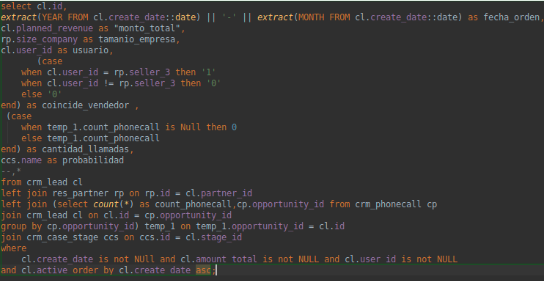
\includegraphics[width=0.5\textwidth]{preprocesamiento/query_extraccion}
    \caption{Query de extraccion}
    \label{fig:query_extraccion}
\end{figure}

\subsection{Preprocesamiento}
\subsubsection{Balanceo}
El balanceo se determinó que la mayoría de datos que eran muertos, solo se tomo 
(cantidad de datos no muertos)*40\% , por ende nos salió que la cantidad de no muertos que seria , debia ser de : 11512
\begin{figure}[H]
    \centering
    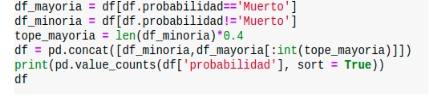
\includegraphics[width=0.5\textwidth]{preprocesamiento/codigo_balanceo}
    \caption{Codigo de balanceo}
    \label{fig:codigo_balanceo}
\end{figure}
La data antes del balanceo : 
\begin{figure}[H]
    \centering
    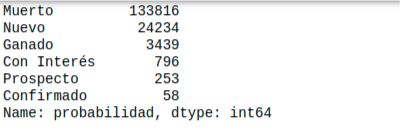
\includegraphics[width=0.5\textwidth]{preprocesamiento/data_antes_balanceo}
    \caption{Data antes del balanceo}
    \label{fig:data_antes_balanceo}
\end{figure}
La data despues del balanceo : 
\begin{figure}[H]
    \centering
    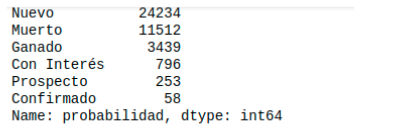
\includegraphics[width=0.5\textwidth]{preprocesamiento/data_despues_balanceo}
    \caption{Data despues del balanceo}
    \label{fig:data_despues_balanceo}
\end{figure}

De lo cual solo quedo 40292 instancias, despues de aplicar el balanceo.

\subsubsection{Limpieza}
Se determino la cantidad de nulos en cada campos.
\begin{figure}[H]
    \centering
    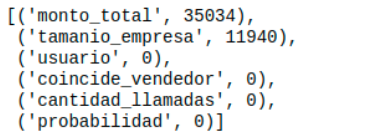
\includegraphics[scale=0.5]{preprocesamiento/cantidad_nulos}
    \caption{Cantidad de nulos}
    \label{fig:cantidad_nulos}
\end{figure}
Por lo que vemos que los nulos estan presentes en los campos
'monto\_total' y 'tamanio\_empresa', por lo que se aplicara la siguiente limpieza:
\begin{itemize}
    \item Al campo 'monto\_total' se reemplazó los nulos por 0 , al ser un valor continuo.
    \item Al campo '    tamanio\_empresa' se reemplazó los nulos al ser un valor discreto.
\end{itemize}

Por lo que el resultado es : 
\begin{figure}[H]
    \centering
    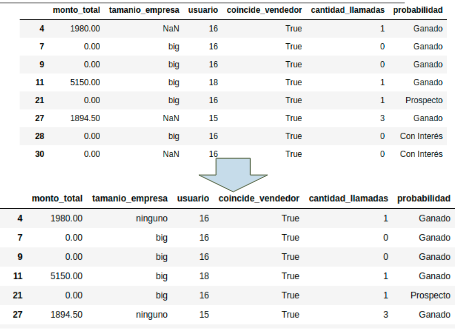
\includegraphics[width=0.5\textwidth]{preprocesamiento/antes_despues_limpieza}
    \caption{Antes y despues de la limpieza de los datos}
    \label{fig:antes_despues_limpieza}
\end{figure}

\subsubsection{Numerización}
Se procedio a numerizar los datos cualitativos. \\
Determinamos un valor por cada valor cuantitativo que tenia cada campo cualitativo. Lo cuales fueron:
\begin{itemize}
    \item tamanio\_empresa:
    \begin{itemize}
        \item big : 3
        \item medium : 2
        \item small : 1
        \item ninguno : 0
    \end{itemize}
    \item coincide\_vendedor:
    \begin{itemize}
        \item True : 1
        \item False : 0
    \end{itemize}
    \item probabilidad:
    \begin{itemize}
        \item Ganado : 100
        \item Confirmado : 80
        \item Prospecto : 60
        \item Con interés: 40
        \item Nuevo: 20
        \item Muerto: 0
    \end{itemize}
\end{itemize}
Por lo que el resultado es : 
\begin{figure}[H]
    \centering
    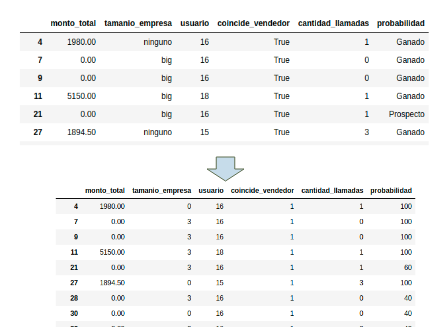
\includegraphics[width=0.5\textwidth]{preprocesamiento/antes_despues_numerizacion}
    \caption{Antes y despues de la numerización de los datos}
    \label{fig:antes_despues_numerizacion}
\end{figure}
\subsection{Correlación}
La correlación de los datos fueron:
\begin{figure}[H]
    \centering
    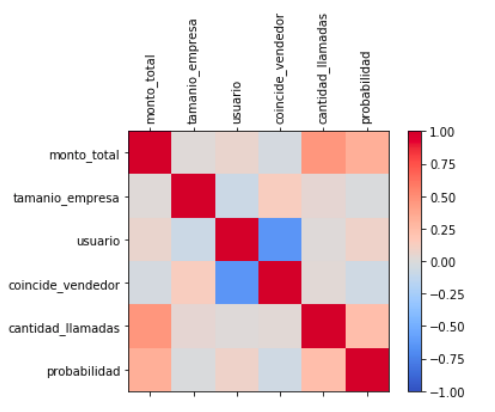
\includegraphics[width=0.5\textwidth]{preprocesamiento/correlacion_datos}
    \caption{Correlación de los datos}
    \label{fig:correlacion_datos}
\end{figure}
Lo cual la correlación que más nos interesa es la de la probabilidad,
puesto que es nuestra variable de predicción del modelo de regresión que estamos 
planteando.
\subsection{Proceso del LSTM}
Se ingresará las variables al LSTM y de acuerdo con el modelo estructurado se predecirá el porcentaje del éxito de la compra.
\begin{figure}[H]
    \centering
    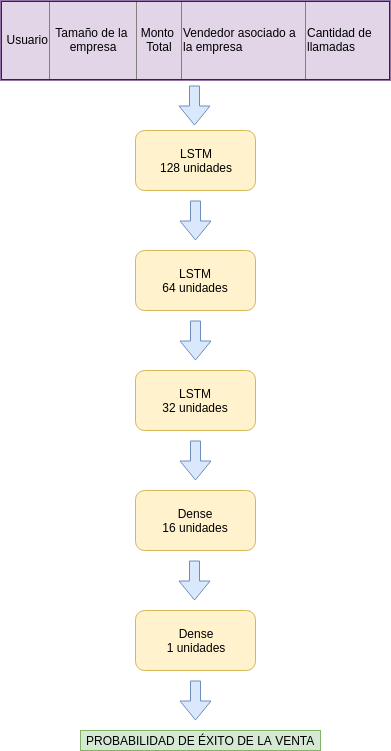
\includegraphics[width=0.5\textwidth,height=14cm]{LSTM}
    \caption{Proceso del LSTM}
    \label{fig:proceso_lstm}
\end{figure}

Se entreno un LSTM por input y se concatenó en una capa oculta de cual el resultado es la probabilidad de ventas.\\
De lo cual la salida del modelo es:
\begin{table}[h]
    \caption{Estructura de la salida del modelo de predicción de ventas.}
    \centering
    \begin{tabularx}{0.4\textwidth} {
            | >{\raggedright\arraybackslash}X
            | >{\centering\arraybackslash}X
            | >{\raggedleft\arraybackslash}X |}
        \hline
        Variable              & Descripcion                             \\
        \hline
        0 a 100\%        & Nos indicara una probabilidad baja de éxito de la compra        \\
        \hline
    \end{tabularx}
    \label{tab3}
\end{table}
\section{RESULTADOS}
El modelo LSTM, utilizando LSTM para predecir el valor continuo de la probabilidad.\\

La configuración del modelo LSTM es:
\begin{itemize}
\item Épocas: 600
\item Batch size (Tamaño de lote): 512
\item Optimizador: adam
\item Primera capa : 128 unidades
\item Segunda capa: 64 unidades
\item Tercera capa: 32 unidades
\item Función de activación en la última capa: relu
\item Función de pérdidas: Error cuadrático medio
\end{itemize}

El modelo fue entrenado con el 75\% de los datos obtenidos y se usó el 25\% de los datos para poder evaluar el modelo.
\begin{figure}[H]
    \centering
    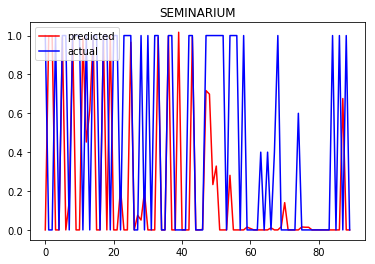
\includegraphics[width=0.5\textwidth]{metricas/prediccion}
    \caption{Predicción de valores de testing}
    \label{fig:prediccion}
\end{figure}
Se puede observar que hay una gran desvariación de la precisión, esto se debe a que el dataset proviene de una empresa real, por lo que la data es muy irregular, además que las variaciones de las ventas, en un entorno real, son muy irregulares en muchos aspectos y esto causa ruido en el modelo.\\
La pérdida fue disminuyendo por cada época que pasaba, por lo cual se ve claramente como esta constante dentro de un rango de valores 0.0015 a 0.0012 (Fig.~\ref{fig:perdida_modelo})
\begin{figure}[H]
    \centering
    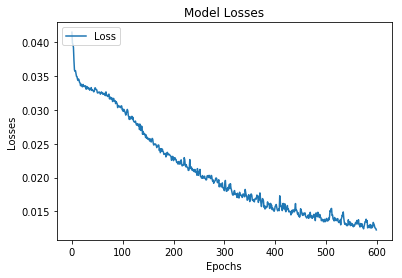
\includegraphics[width=0.5\textwidth]{metricas/perdida}
    \caption{Pérdida del modelo}
    \label{fig:perdida_modelo}
\end{figure}
De igual manera el error medio absoluto porcentual también se nota constante, aunque haya a veces pequeñas fluctuaciones, debido obviamente algunas fluctuaciones muy distante (Fig.~\ref{fig:mae_modelo})
\begin{figure}[H]
    \centering
    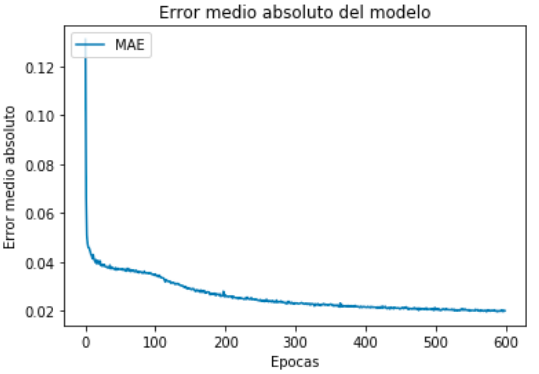
\includegraphics[width=0.5\textwidth]{metricas/mean_absolute_error}
    \caption{Error medio absoluto del modelo}
    \label{fig:mae_modelo}
\end{figure}
Por ultimo error de la raíz del error cuadrático medio también se nota constante ( Fig. ~\ref{fig:rmse_modelo})
\begin{figure}[H]
    \centering
    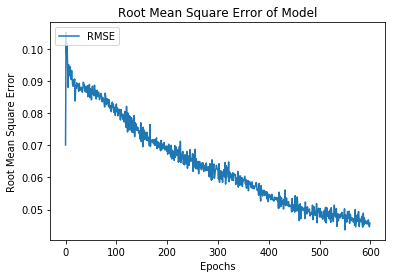
\includegraphics[width=0.5\textwidth]{metricas/rmse}
    \caption{Raíz del error cuadrático medio del modelo}
    \label{fig:rmse_modelo}
\end{figure}
Entonces los resultados finales son :
\begin{table}[h]
    \caption{Resultados del modelo}
    \centering
    \begin{tabularx}{0.4\textwidth} {
            | >{\raggedright\arraybackslash}X
            | >{\centering\arraybackslash}X
            | >{\raggedleft\arraybackslash}X |}
        \hline
        Métrica              & Resultado                             \\
        \hline
        Perdida o Error cuadrático medio     & 0.0066        \\
        \hline
        Error medio absoluto    & 0.0200       \\
        \hline
        Error de la raíz cuadrada de la media    & 0.0200       \\
        \hline
    \end{tabularx}
    \label{tab3}
\end{table}

\section{APLICATIVO}
Se desarrollo un aplicativo Web , que esta constituido por :
\begin{itemize}
    \item BackEnd : Se desarrollo en Flask , y las librerias que usan son :
    \begin{itemize}
        \item keras
        \item blueprints
        \item tensorflow
    \end{itemize}
    \item FrontEnd: Se desarrollo en ReactJS , del cual consume al backend.
\end{itemize}

Y el resultado fue:
\begin{figure}[H]
    \centering
    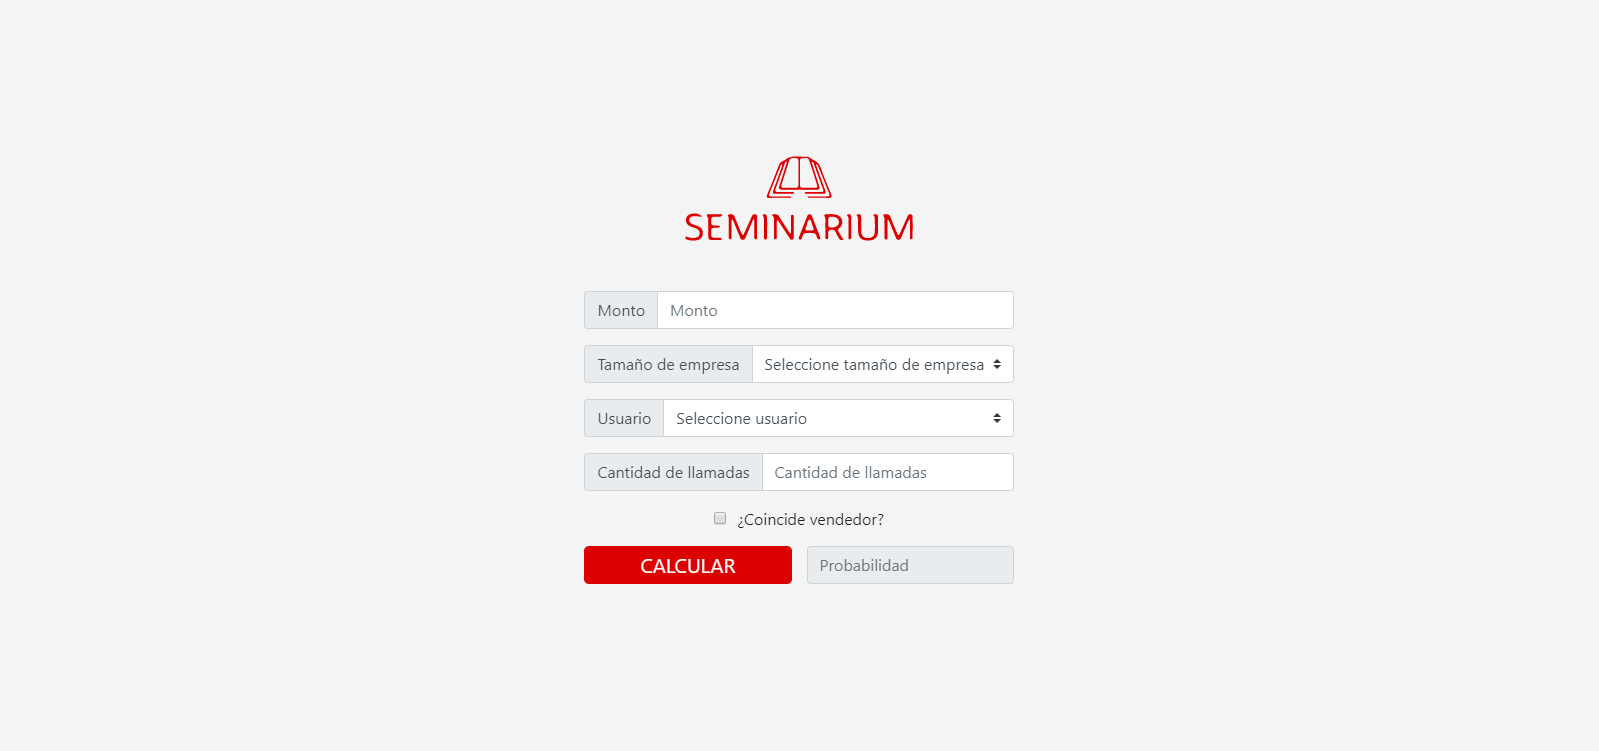
\includegraphics[width=0.5\textwidth]{aplicativo/sin_datos}
    \caption{Aplicativo Web sin Datos}
    \label{fig:aplicativo_sin_datos}
\end{figure}
\begin{figure}[H]
    \centering
    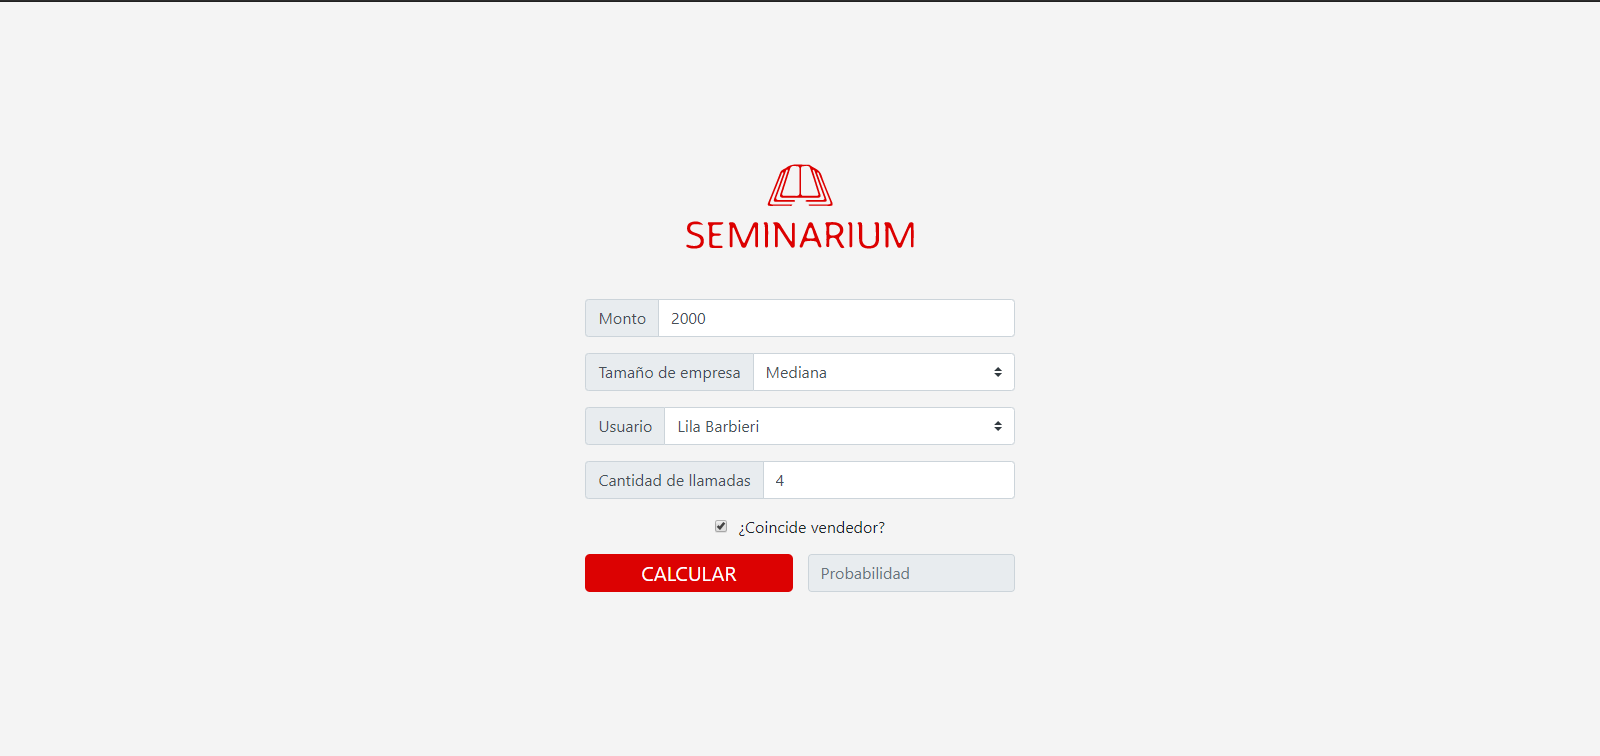
\includegraphics[width=0.5\textwidth]{aplicativo/con_datos}
    \caption{Aplicativo Web con Datos}
    \label{fig:aplicativo_con_datos}
\end{figure}
\begin{figure}[H]
    \centering
    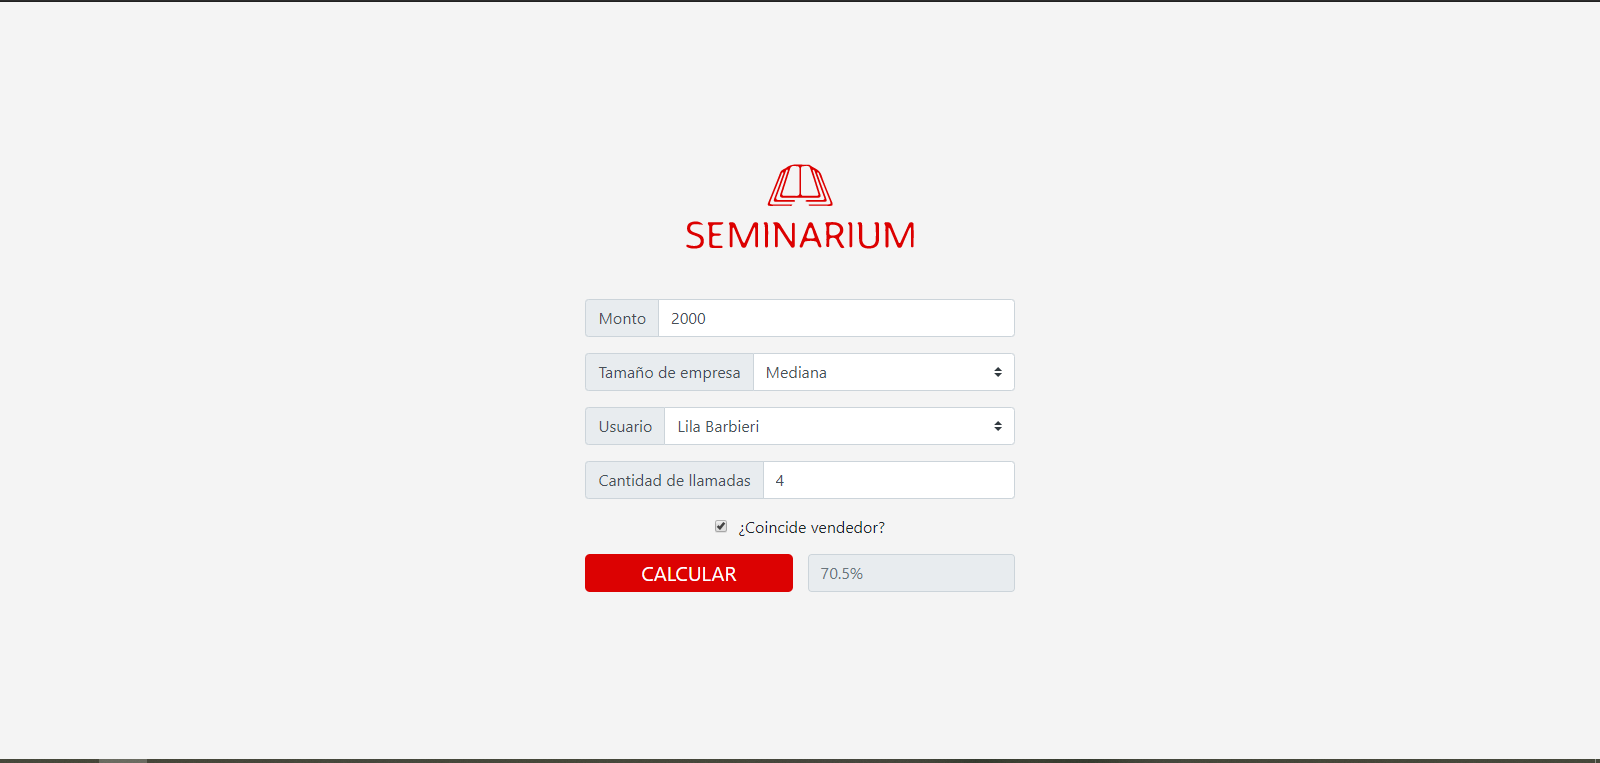
\includegraphics[width=0.5\textwidth]{aplicativo/con_datos_resultado}
    \caption{Aplicativo Web con Datos y Resultado}
    \label{fig:aplicativo_con_datos_resultado}
\end{figure}



\section{DISCUSION}
Las investigaciones \cite{b3}, \cite{b4} (data de apple - data.world) , \cite{b20} usan el monto total obtenido en una serie de tiempo  , otros como \cite{b22} usan algunos datos de ventas , pero solo en el contexto de ventas de moda e incluso alguno como \cite{b24} agregaban análisis de sentimientos. Pero la fuente principal de una venta es el cliente y sobre todo datos tan relevantes como el tamaño de la empresa, sus ventas anteriores e incluso si esta fidelizado con la vendedora. Por lo que el dataset de esta investigación se concentra precisamente en esos datos que en otras investigaciones no han tomado en cuenta.\\
Después de entrenar el modelo LSTM que predice el éxito de la venta es necesario hacer una comparación del desempeño con otras soluciones ante el problema de predicción de ventas pero en la investigación que se ha realizado hemos detectado que muchos de los autores hablan de la predicción de ventas como el monto total ganado de la venta en un periodo de tiempo\cite{b2}\cite{b5}\cite{b6} que logran entre 95\% a 98\% de precisión, algunos otros hablan de la predicción de flujo de clientes\cite{b11}\cite{b12}\cite{b13}\cite{b14} que logran entre 80\% a 85\% de precisión  e incluso algunos han juntado datos del producto\cite{b1} con las de venta  en el cual se mide con la métrica R2 que logra un 0.727 , pero ninguno habla de éxito de la predicción de la venta de forma individual contando con las variables de la venta como la del cliente por lo que en esta investigación se desarrolló la predicción de la venta de forma individual del cual el resultado es probabilidad de éxito de la venta y esto permitirá que tanto la gerencia comercial como la gerencia de marketing puedan analizar y “atacar” las ventas de forma más precisa.\\
En las principales investigaciones de ventas \cite{b2}\cite{b5}\cite{b6}\cite{b1} se enfocan en el monto real que se ganaría durante una serie temporal (Año, mes e incluso día), pero no cuentan muchas variables de un entorno real, y además es muy general el monto ganado, de lo cual surge dos grandes preguntas:
\begin{itemize}
\item ¿De cómo se ganó ese monto ganado?
\item ¿Como puedo mejorar ese monto ganado?
\end{itemize}
Obviamente las investigaciones de ventas no atacan estas dos preguntas como tal, esto causa de que la empresa no sepa exactamente como mejorar en las ventas y además que tampoco sepa que estrategias poder desplegar, tanto de marketing como comercial. Por lo que en esta investigación tratamos de resolver esos problemas, dando un enfoque más preciso de la venta de forma individual y el éxito que se puede lograr de ella.\\
Las investigaciones \cite{b3}\cite{b4} que nos comentan que los modelos híbridos son los más usados en problemas que normalmente una sola técnica de machine learning o deep learning no puede resolverlo, pero el mundo del análisis predictivo de la venta ha sido muy poco usado los híbridos puesto que muchas investigaciones solo se han enfocado en predecir la ganancia total que se generará en un periodo de tiempo; por lo que realizar este análisis en función de otras variables resulta más complejo y se necesita de un modelo más complejo, por eso en esta investigación se optó por el uso de modelo LSTM para determinar el éxito de una venta tomando en cuenta otras variables que otras investigaciones han omitido.\\
El desarrollo de modelos en escenarios reales es más complicado por la gran cantidad de datos “sucios” lo que causara mucho ruido sino se lograr un óptimo preprocesamiento y limpieza de estos.

\section*{CONCLUSIÓN Y TRABAJO FUTURO}
Se determino que los mejores modelos de predicción para ventas son modelos basados en Deep learning . Por ende se desarollo un modelo LSTM para determinar el éxito de una venta tomando en cuenta otras variables que otras investigaciones han omitido. Y tambien el desarrollo de modelos en escenarios reales es más complicado por la gran cantidad de datos “sucios” lo que causara mucho ruido sino se lograr un optimo preprocesamiento y limpieza de estos.\\
Se podría utilizar otros híbridos para manejar variables de ventas en conjunto con las variables del cliente. Y tambien se podria obtener nuevos datos provenientes de otros giros de negocios de ventas para mejorar la cobertura del modelo y no solo empresas B2B.
\begin{thebibliography}{00}
    \bibitem{b1} V. L. F. S. A.L.D.Loureiro, "Exploring the use of deep neural networks for sales forecasting in fashion retail", Decision Support Systems, pp. 81-93, 2018.
    \bibitem{b2} M. Müller-Navarra, S. Lessmann y S. Voß, "Sales Forecasting with Partial Recurrent Neural Networks: Empirical Insights and Benchmarking Results", de 2015 48th Hawaii International Conference on System Sciences, Kauai, HI, USA, 2015.
    \bibitem{b3} H. Y. Y. G. Z. Z. Shenjia Ji, "Research on Sales Forecasting Based on ARIMA and BP Neural Network Combined Model", de Proceedings of the 2016 International Conference on Intelligent Information Processing, Wuhan, China, 2016.
    \bibitem{b4} S. P. K. J. L. A. J. S. G. U. G. Rankothge Gishan Hiranya Pemathilake, "Sales Forecasting Based on AutoRegressive Integrated Moving Average and Recurrent Neural Network Hybrid Model", de 2018 14th International Conference on Natural Computation, Fuzzy Systems and Knowledge Discovery, Huangshan, China, China, 2018.
    \bibitem{b5} R. S. ,. S. Vicky Chrystian Sugiarto, "Sales forecasting using Holt-Winters in Enterprise Resource Planning at sales and distribution module", de 2016 International Conference on Information \& Communication Technology and Systems (ICTS), Surabaya, Indonesia, 2016.
    \bibitem{b6} H. Y. H. C. L. W. H. W. X. Z. X. L. Tong Chen, "TADA: Trend Alignment with Dual-Attention Multi-Task Recurrent Neural Networks for Sales Prediction", de International Conference on Data Mining, Brisbane,Australia, 2018.
    \bibitem{b7} C. Gallagher, M. G. D’Arcy y M. Brian, "A Bayesian Classification Approach to Improving Performance for a Real-World Sales Forecasting Application", de 2015 IEEE 14th International Conference on Machine Learning and Applications, Miami, FL, USA, 2015.
    \bibitem{b8} Y.-S. W. H.-Y. K. J.-Y. T. ,. C.-C. C. H.-. Kuen-Han Tsai, "Multi-Source Learning for Sales Prediction", de 2017 Conference on Technologies and Applications of Artificial Intelligence, Taipei, Taiwan, 2017.
    \bibitem{b9} L. T. V. R. Xin Xu, "Hitting your number or not? A robust \& intelligent sales forecast system", de 2017 IEEE International Conference on Big Data (Big Data), Boston, MA, USA, 2017.
    \bibitem{b10} J. Z. X. Z. Zongming Yin, "Forecast customer flow using long short-term memory networks", de 2017 International Conference on Security, Pattern Analysis, and Cybernetics (SPAC), Shenzhen, China, 2017.
    \bibitem{b11} L. Kuo-Yi y J. Jeffrey, "A Deep Learning-Based Customer Forecasting Tool", de 2016 IEEE Second International Conference on Multimedia Big Data (BigMM), Taipei, Taiwan, 2016.
    \bibitem{b12} K. Y. Yuta Kaneko, "A Deep Learning Approach for the Prediction of Retail Store Sales", de 2016 IEEE 16th International Conference on Data Mining Workshops, Barcelona,Spain, 2016.
    \bibitem{b13} A. N. A. H. I. P. Eric Michael Smith, "Forecasting Customer Behaviour in Constrained E-Commerce Platforms", de 8th   International Conference of Pattern Recognition Systems (ICPRS 2017), Madrid, Spain , 2017.
    \bibitem{b14} R. Jia, R. Li, M. Yu y S. Wang, "E-commerce purchase prediction approach by user behavior data", de 2017 International Conference on Computer, Information and Telecommunication Systems (CITS), Dalian, China, 2017.
    \bibitem{b15} V. C. Sugiarto, R. Sarno y D. Sunaryono, "Sales Forecasting Using Holt-Winters in Enterprise Resource Planning At Sales and Distribution Module", de 2016 International Conference on Information, Communication Technology and System (ICTS), Surabaya, Indonesia, 2016.
    \bibitem{b16} B. Suh, "Sales Teams Aren’t Great at Forecasting. Here’s How to Fix That.", 19 Marzo 2019. [En línea]. Available: https://hbr.org/2019/03/sales-teams-arent-great-at-forecasting-heres-how-to-fix-that .
    \bibitem{b17} B. Hedayati, "How To Access Intelligence: Data-Driven Transformation In Marketing Operations", 10 Abril 2019. [En línea]. Available: https://www.forbes.com/sites/forbestechcouncil/2019/04/10/how-to-access-intelligence-data-driven-transformation-in-marketing-operations/\#7dff34a35a33.
    \bibitem{b18} L. Bullock, "Content Marketing Lead Generation Tactics That Actually Work In 2019", 28 Marzo 2019. [En línea]. Available: https://www.forbes.com/sites/lilachbullock/2019/03/28/content-marketing-lead-generation-tactics-that-actually-work-in-2019/\#653239c46c0c.
    \bibitem{b19} V. Antonio, "How AI Is Changing Sales", 30 Julio 2018. [En línea]. Available: https://hbr.org/2018/07/how-ai-is-changing-sales.
    \bibitem{b20} Y. K. P. S. S. U. ,. V. S. a. S. B. Mohit Gurnani, "Forecasting of sales by using fusion of Machine Learning techniques", de 2017 International Conference on Data Management, Analytics and, Pune, India, 2017.
    \bibitem{b21} S. Ren, T.-M. Choi y N. Liu, "Fashion Sales Forecasting With a Panel Data-Based Particle-Filter Model", IEEE Transactions on Systems, Man, and Cybernetics: Systems, vol. 45, nº 3, pp. 411-421, 2015.
    \bibitem{b22} P.C.L.Hui y T.-M.Choi, "Using artificial neural networks to improve decision making in apparel supply chain systems", Information Systems for the Fashion and Apparel Industry, nº 5, pp. 97-107, 2016.
    \bibitem{b23} Z. L. K. Rotenberg, "Sales Forecasting Methods", 2014. [En línea].
    \bibitem{b24} M. J. Schneider y S. Gupta, "Forecasting sales of new and existing products using consumer reviews : A random projections approach", International Journal of Forecasting, vol. 32, nº 2, pp. 243-256, 2016.

\end{thebibliography}
\end{document}